\subsection{Design av kolonnefamiliedatabasen}
Her brukte vi datasettet "World University Rankings" med Times Higher Education World University Ranking metodikken fra Kaggle:

https://www.kaggle.com/mylesoneill/world-university-rankings?select=timesData.csv

\subsubsection{Begrunnelse bak valgene rundt kolonnefamilie- og grafdatabase}
Raske queries, vi vil gjerne vite om alle skoler basert på forskjellige faktorer, og vi ønsker å gjøre det 
mange ganger med forskjellige variabler. I tillegg hjelper det spesielt at en kan selv velge grad av 
konsistens ved en read/write. En kan altså her velge selv hvor mange av nodene en write skal kjøres 
på, og replikering av nodene kan gjøres etter behov. Skalerbarheten er altså massiv, og når det 
kommer hyppig med queries, så vil det ikke nesten ikke merkes.

\subsubsection{Hvorfor kolonnedatabase?}
Grunnen til at vi har valgt kolonnedatabase for dette datasettet er blant annet fordi 
kolonnedatabaser tilbyr svært rask lesing og og skrive-spørringer. Dette er nyttig, siden vi bruker et 
stort datasett med mange rader. I tillegg er kolonnefamiliedatabaser mer egnet for AP-systemer, 
som vil si at den prioriterer tilgjengelighet over konsistens. Dataen i dette datasettet oppdateres ikke 
ofte (maksimalt en gang i året), og ved hjelp av timestamps for hver verdi vil ikke konsistensen være 
et stort bekymring

\subsubsection{Operasjoner}
Create
INSERT INTO <table name>
(<column1>, <column2>....)
VALUES (<value1>, <value2>...)
USING<option>

Read
SELECT * FROM <table name>;

Delete
DELETE <identifier> FROM <table name> WHERE <condition>;

\subsubsection{Hvordan eksisterende data oppdateres}
\begin{itemize}
  \item Ny data kommer inn
  \item Data/kommando verifisering
  \item Sjekker om raden er ledig
  \item Ledig - oppdaterer raden
  \item Ikke ledig - lager ny rad for samme data
  \item Data oppdateres på aktuelle noder
\end{itemize}

\subsubsection{Dataobjekter}
% Aggregering 1 %
\textbf{Rådata}\\
Dette dataobjektet representerer rådata brukes til å oppdatere dataen i databasen. Dette objektet 
opprettes når ny data blir lest inn, eller når bruker legger inn selv.

\FigureCounter
\begin{figure}[H]
  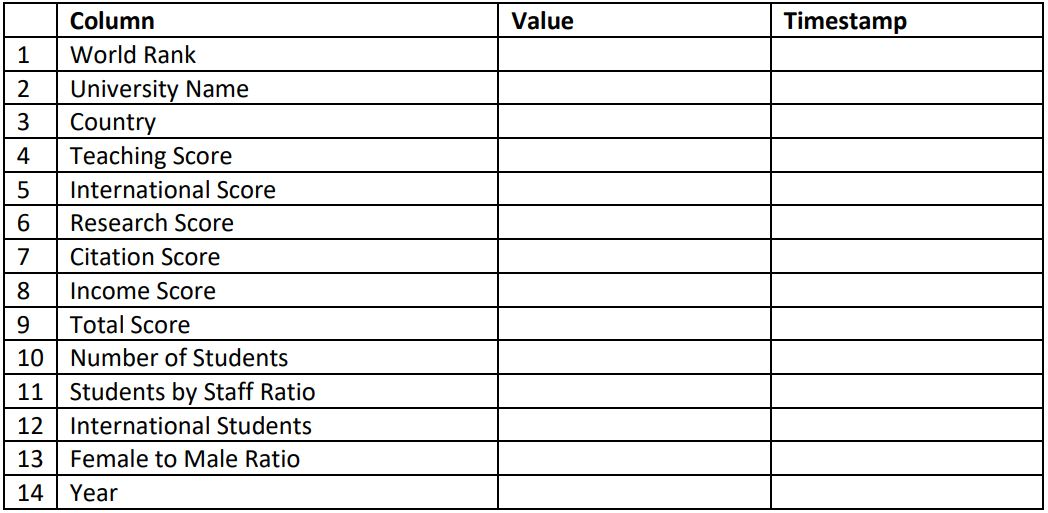
\includegraphics[width=\textwidth]{images/milepael4/rawObject.JPG}
\end{figure}

\textbf{Pseudo-Kode}
\begin{enumerate}
  \item Register each field from user input
  \item Save data as an object
  \item Post object to database
\end{enumerate}

% Aggregering 2 %
\textbf{Top 10 Universities By Diversity}\\
I dette dataobjektet rangeres hvert universitet ut ifra en ny faktor som vi har skapet kalt "Diversity 
Score". Dette er en sammenslåing av følgende felt fra Rådata-objektet: Number of Students, 
International Students, Female To Male. På denne måten kan man få en oversikt over hvilke skoler 
som har mest mangfoldig studentmiljø. Til slutt skal dette ha en limit på 10.

\FigureCounter
\begin{figure}[H]
  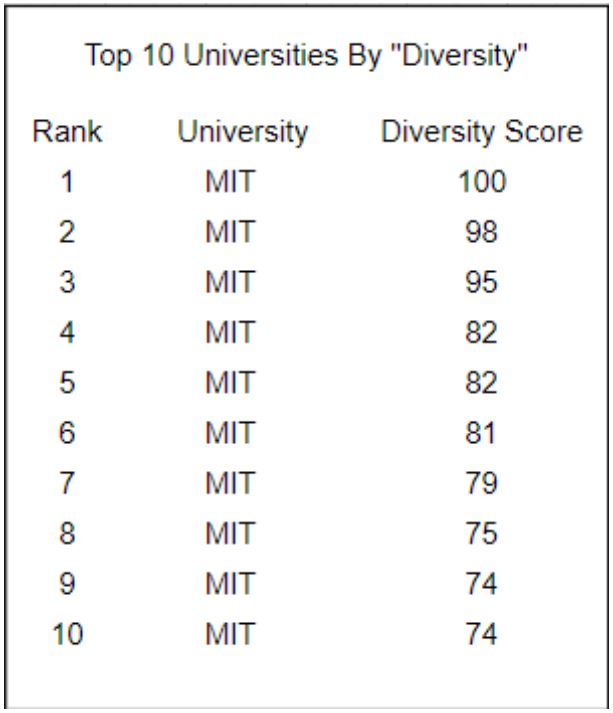
\includegraphics[scale=1]{images/milepael4/topTenUnis.JPG}
\end{figure}

\textbf{Pseudo-Kode}
\begin{enumerate}
  \item Calculate diversity factor
  \item Group By University
  \item Limit by 10
\end{enumerate}
\pagebreak
% Aggregering 3 %
\textbf{Average Total Score By Number Of Students}\\
Dette objektet visualiserer total score innenfor hvert intervall of studentmengder. Dette kan være 
interessant for å se om kvaliteten på universitetet.

\FigureCounter
\begin{figure}[H]
  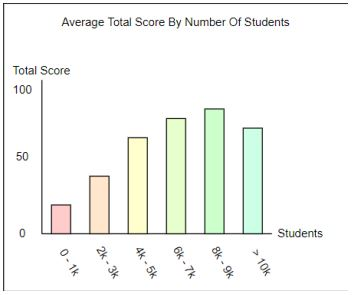
\includegraphics[scale=1]{images/milepael4/averageScoreByStudents.JPG}
\end{figure}

\textbf{Pseudo-Kode}
\begin{enumerate}
  \item Calculate average total score
  \item Define number of students interval
  \item Group by number of students interval
\end{enumerate}